\RequirePackage[T1]{fontenc}
\documentclass[conference]{IEEEtran}
\usepackage{cite}
\usepackage{amsmath,amssymb,amsfonts}
\usepackage{graphicx}
\usepackage{textcomp}
\usepackage{xcolor}
\usepackage{booktabs}
\usepackage{url}
\usepackage{xspace}

\newcommand{\sys}{Pacta\xspace}
\newcommand{\cert}{\mathsf{Cert}}
\newcommand{\qsem}[1]{[\![#1]\!]}
\newcommand{\hash}{\mathsf{H}}
\newcommand{\pol}{\mathsf{pol}}
\newcommand{\ans}{\mathsf{Ans}}
\newcommand{\desc}{\mathsf{Desc}}
\newcommand{\man}{\mathsf{Man}}
\newtheorem{definition}{Definition}
\newtheorem{lemma}{Lemma}
\newtheorem{theorem}{Theorem}
\setlength{\textfloatsep}{6pt plus 1pt minus 2pt}
\setlength{\floatsep}{5pt plus 1pt minus 2pt}
\setlength{\intextsep}{5pt plus 1pt minus 2pt}
\setlength{\abovecaptionskip}{2pt}
\setlength{\belowcaptionskip}{0pt}
\renewcommand{\arraystretch}{0.94}

\begin{document}

\title{Pacta: Certifying Evidence Plans for Governed Analytical Queries}

\author{
\IEEEauthorblockN{Haoyi Zhang, Huaijin Ran}
\IEEEauthorblockA{\textit{Xi'an Jiaotong-Liverpool University}\\
Suzhou, China\\
\{hyeliozhang, seventeen17510\}@gmail.com}
}

\maketitle

\begin{abstract}
Governed analytics changes the unit of query-result verification. An answer may be authentic for a table snapshot and still be wrong for the tenant, purpose, policy release, projection, version, or row predicate that defines the client's permitted query. We present \sys, a certifying query processor that makes the governed request itself the object of authentication. \sys defines correctness as equality to a query over a manifest-derived authorized bag, and implements evidence plans whose typed proof objects discharge request binding, descriptor conservation, policy binding, projection safety, omission completeness, freshness, and disclosure obligations. The system combines schema-bound descriptor trees with typed dimension attributes, policy-cube and prefix-cube summaries, opened-row and opened-multiset fallbacks, signed descriptor catalogs, and a certifying optimizer that rejects cheap plans missing verifier obligations before ranking sound alternatives. The implemented boundary covers range selection/projection, group-by count/sum/derived average/HAVING, exact count-distinct, threshold top-k with ties, returned-pair joins, complete foreign-key joins, complete anti-joins, complete many-to-many expansion joins, and open-scan fallback for unsummarized deterministic predicates. In the full-baseline matrix, \sys group-by certificates have 31.4 KiB median size, 3.64 ms generation, and 1.98 ms client verification. At larger scale, a 1M-row page-cube certificate verifies in 84.83 ms, while a 50K-row authenticated prefix cube verifies range group-by certificates in 2.89 ms with 22.5 KiB proofs. The optimizer exposes a 59x proof-size frontier between sound compact summaries and sound opened evidence, and rejects the compact plan for row predicates whose attributes were not committed by the summary. The artifact ties these claims to descriptor-only verification, leakage contracts, SQLite semantic oracles, adversarial mutation tests, versioned updates, public tabular mappings, robustness sweeps, and page/prefix-cube physical layouts.
\end{abstract}

\begin{IEEEkeywords}
Authenticated query processing, governed data sharing, query result verification, policy-aware query processing, physical database design, provenance
\end{IEEEkeywords}

\section{Introduction}
A governed analytics service can be wrong even when every returned row is authentic. Consider a dashboard server that answers a regional audit query over the correct table root but under yesterday's manifest, a broader tenant predicate, or a projection mask that hides the attribute needed to check policy. The rows and aggregates may have valid membership proofs, yet the released answer is not the answer to the query the client was allowed to ask. This is the central mismatch addressed by \sys: governed sharing needs result verification for the effective policy-bound query, not only for the base relation.

Organizations increasingly expose data through outsourced analytics, multi-tenant dashboards, data-product APIs, clean rooms, governed open-data releases, and data marketplaces. These systems answer group-by tables, ranked lists, filtered reports, and audit drill-downs under policies about tenant, purpose, region, consent, sensitivity, projection, retention, and release class. A row-level proof authenticates contributors; a provenance explanation explains returned contributors; a policy log records an enforcement decision. None of these objects alone proves that every authorized contributor was included, every unauthorized contributor was excluded, and the request, projection, manifest release, and version matched the client's contract.

Authenticated data structures and outsourced databases provide a deep foundation for verifying query results~\cite{devanbu2003authentic,martel2004model,tamassia2003ads,pang2004edge,pang2005completeness,mykletun2004outsourced,sion2005assurance,li2006dynamic,li2010aggregation,papadopoulos2009sae,papadopoulos2010streams,chen2013topk}. Access-control, purpose-based policy, and view-based systems provide a separate foundation for defining authorized data~\cite{stonebraker1974access,rizvi2004fgac,kabra2006fgac,chaudhuri2007predicated,byun2008purpose,colombo2015action,sandhu1996rbac,jajodia1997multipolicy}. Provenance systems explain why outputs depend on inputs~\cite{cui2000lineage,buneman2001whywhere,green2007semiring,cheney2009provenance,glavic2021provenance}. Governed analytics needs these lines to meet at the result boundary. The verifier must check not only that returned tuples are authentic, but that the returned answer is exactly the query answer over the manifest-derived authorized relation.

\sys addresses this problem with \emph{policy-carrying query certificates}. A certificate binds six objects: the relation descriptor, the policy-manifest descriptor, the client-visible request digest, the effective query, the returned answer, and omission evidence for authorized non-returned tuples. The central idea is to make policy a first-class part of the authenticated query contract. Each covered index node commits not only to a hash, but also to a key interval, cardinality, ordered child descriptors, and a policy-cube summary. The verifier derives the effective policy from the committed manifest, verifies the descriptor chain, folds only authorized contributions, and rejects certificates that change the query, policy, projection, or version.

Fig.~\ref{fig:semantics} shows the workflow. A data owner publishes a relation descriptor and a policy-manifest descriptor. A server returns an answer and a certificate. A verifier reconstructs the effective governed query and checks the answer against the descriptors. The policy system remains ordinary database metadata; the contribution is that the metadata becomes part of the result-verification semantics.

\begin{figure}[t]
\centering
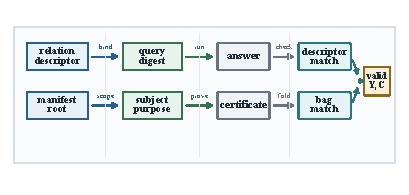
\includegraphics[width=\linewidth]{figs/semantics_pipeline.pdf}
\caption{Policy-carrying query-result verification. The checked object is the answer to a query under a specific manifest, subject, purpose, projection, and relation version.}
\label{fig:semantics}
\end{figure}

\textbf{Contributions.} First, \sys defines governed analytical correctness as request-bound equality over a committed authorized bag: schema, duplicate semantics, projection mask, descriptor-typed join attributes, subject-purpose policy, manifest release, and relation version are verifier inputs. Second, it gives a typed certificate algebra whose evidence objects state exactly which completeness obligation they discharge. Third, it introduces descriptor-bound policy-cube indexes and a certifying optimizer that enumerates physical evidence plans, rejects candidates missing verifier obligations, and chooses among compact summaries, tuple/frontier proofs, opened ranges, opened multisets, top-k accumulators, and join witnesses. Fourth, it implements the supported verification boundary: canonical contract IR, strict descriptor-only client verification, signed catalog freshness, executable leakage contracts, SQLite oracles, mutation tests, versioned updates, public profile mappings, page-cube and prefix-cube physical layouts, and cost-frontier experiments that distinguish sound compact plans from compact inadmissible ones.

The paper is data-engineering-first: the research object is the database contract connecting query semantics, physical evidence plans, verifier obligations, and scale-aware evidence choice. Cryptographic hashes provide tamper evidence, but the central systems question is which relational expression is certified, which summary or opened witness proves it, and how an optimizer can trade proof size, verification time, build cost, and update footprint without changing the governed answer.

\section{Governed Query Contract}
\subsection{Model and Certification Boundary}
We consider a data owner, an untrusted query server, and a verifier used by a consumer or auditor. The owner maintains versioned relations $R_v$ and policy manifests $M_v$. For each committed version, the owner publishes a signed catalog entry for descriptor $D_v$ containing a relation root, a relation-descriptor digest, a manifest root, a schema contract, a version number, and a monotone freshness epoch. The server stores relations, indexes, and policy metadata, executes queries, and returns result/certificate pairs. The verifier knows the owner public key, query, subject, purpose, expected descriptor, and verification algorithm.

The server may return wrong aggregates, omit authorized tuples, add unauthorized tuples, compute under a widened or narrowed policy, change a projection mask, reuse an old version, substitute a neighboring range, or relabel a boundary subtree. The server cannot find collisions in the hash function or forge a signed owner descriptor. The owner-side policy compiler, manifest publication path, and client verifier are trusted; validating whether the owner's policy is legally or organizationally correct is outside the cryptographic certificate boundary. This follows the standard authenticated outsourced database setting~\cite{hacigumus2002das,pang2004edge,sion2005assurance,li2006dynamic}, extended from data authenticity to governed query semantics.

The certified property is result integrity for governed analytics: authenticity, omission completeness, manifest-derived policy binding, projection safety, and version freshness. \sys does not claim confidentiality, differential privacy, hidden access patterns, or arbitrary SQL verification; encrypted query processing, trusted hardware, or privacy mechanisms can be layered when a deployment needs those properties~\cite{hacigumus2002encrypted,popa2011cryptdb,zheng2017opaque,dwork2006dp}. SQL support is expressed as typed certification contracts. A visible query may be executed by a richer engine, but an auditable release is accepted only when it compiles to a verifier-supported contract with explicit evidence obligations; unsupported SQL, nondeterministic predicates, uncommitted UDFs, and out-of-manifest policy rules fail closed.

\subsection{Effective Governed Semantics}
Let $R_v$ be a relation at version $v$. A manifest maps subject $s$ and purpose $u$ to a predicate $P_{s,u}$ and projection mask $A_{s,u}$. For a query with selection predicate $\theta$, grouping keys $G$, distributive aggregates $F$, and output attributes $A$, the governed expression is
\begin{equation}
Q^{\pol}_{s,u}(R_v)=\pi_{A\cap A_{s,u}}\,\gamma_G^F\,\sigma_{\theta\wedge P_{s,u}}(R_v).
\end{equation}
A result $Y$ is correct exactly when $Y=\qsem{Q^{\pol}_{s,u}(R_v)}$. The release mask is lifted to the output schema: attributes used only for policy, grouping, joins, or aggregate verification may appear inside evidence only under the declared disclosure contract, not as extra released answer columns. The equation is simple, but it changes the verification target. The verifier must not verify $Q(R_v)$ and then assume that policy enforcement happened earlier. It must verify the effective governed query.

\begin{definition}[Governed certificate soundness]
A certificate for $(R_v,M_v,s,u,Q,Y)$ is sound if every accepting verifier run implies: (i) the accepted request digest equals the client-visible governed query contract; (ii) every tuple or summary contributing to $Y$ is committed by the expected schema-bound relation descriptor; (iii) every tuple, joined tuple, or aggregate state required by the operator contract contributes exactly once to the verifier's reconstruction: all authorized in-range tuples for range aggregates and projections, all authorized rows above the top-k cutoff including ties, and all fact/dimension/tag or absence witnesses required by join contracts; (iv) duplicate elimination occurs only for explicit distinct contracts; (v) no tuple violating $P_{s,u}$ or the projection mask contributes to the released result; (vi) the policy was derived from the expected manifest and subject-purpose pair; and (vii) the relation version is the expected version.
\end{definition}

Table~\ref{tab:scope} is part of the claim. It states the implemented SQL-style fragment and the precise obligation for each operator. Selection, projection, range, group-by count/sum, exact count-distinct, row-local open-scan predicates, and group-by HAVING have completeness; average is certified as an exact quotient over the verified count/sum state. Top-k is verified through an accumulator-backed threshold certificate over a sorted score attribute, including ties. Joins have four contracts: returned-pair authenticity for drill-downs with scalar dimension filters such as segment hashed into the request digest, a complete key-foreign-key witness that opens every authorized fact in the range and proves its dimension tuple under explicit dimension predicates, a complete anti-join witness that proves absence of an active matching dimension tuple for every contributing fact, and a complete many-to-many witness that proves both the authorized fact multiset and every tag-side multiset for the touched join keys. This gives reviewers a concrete executable target rather than an ambiguous SQL slogan.

\begin{table}[t]
\centering
\caption{Implemented governed-query contract. Every accepted operator has an explicit evidence obligation.}
\label{tab:scope}
\scriptsize
{\setlength{\tabcolsep}{2pt}
\begin{tabular}{@{}p{0.25\linewidth}p{0.69\linewidth}@{}}
\toprule
Feature & Verified obligation \\
\midrule
Schema/bag contract & Primary-key uniqueness, required non-null verification attributes, descriptor-typed dimension fields, relation version, and manifest release are bound. \\
Selection/\newline projection & Tuple authenticity, mask binding, and complete opened-row coverage for the certified range or projection contract. \\
Range predicate & Complete cover of the indexed key interval plus authenticated frontier descriptors. \\
Row-local predicate & Complete open-range scan authenticates every row in the indexed range before applying an unsummarized deterministic predicate. \\
Group-by/AVG/\newline HAVING & Aggregate equality over authorized leaves and summaries; avg and HAVING are derived from the verified group state. \\
Exact count-distinct & Opened authorized multiset plus primary-keyed row accumulator proves duplicate elimination over committed distinct-key values. \\
Threshold top-k & Request predicate, stable score/primary-key order, exact candidate accumulator, returned rows, and all authorized ties above the certified cutoff. \\
Request/policy filter & Client request digest plus manifest-derived subject-purpose predicate, not a trusted server filter. \\
Returned-pair join & Authenticity and predicate validity for each returned fact/dimension pair, plus request-bound scalar dimension filters. \\
Complete FK join & Completeness for a key-foreign-key range join by opened fact multiset, dimension proofs, and summary fingerprint. \\
Complete anti-join & Completeness for NOT EXISTS by fact multiset plus per-key dimension absence witnesses. \\
Complete M:N join & Completeness for category-expansion joins by fact-multiset evidence and tag-side range witnesses. \\
Catalog freshness & Signed descriptor epoch binds relation version, manifest release, relation descriptor digest, and manifest root. \\
Versioned updates & Non-key leaf-to-root repair; insert, delete, and key-update version rebuilding. \\
Disclosure contract & Each plan declares the fields it opens; verifier-side leakage checks reject evidence outside the release contract. \\
Evidence planning & Chooses only admissible proof shapes: compact summaries, tuple/frontier proofs, opened ranges, opened multisets, top-k accumulators, and join/anti-join witnesses. \\
\bottomrule
\end{tabular}
}
\end{table}

\subsection{Example}
A regional auditor requests sales totals by category for days 200--260. The manifest says that this subject and purpose may see only one tenant, approved regions, sensitivity at most two, and aggregate attributes. The correct answer is not the query over the base relation; it is the query over the authorized slice. A tuple proof for returned rows proves membership, but it does not prove that an in-range unauthorized row was excluded for a policy reason, that an out-of-range authorized row was excluded for a range reason, and that a different tenant's row was excluded for a tenant reason. A provenance list leaves the same uncertainty. A \sys certificate authenticates a cover of the range, binds the manifest-derived predicate, and folds only authorized contributions into the answer.

This example exposes the design requirement. The certificate cannot be only a list of returned rows. It must include omission evidence, policy evidence, and projection evidence. Conversely, it should not materialize the whole table when a compact summary is sufficient. The problem is therefore not merely to add a Merkle path to each row; it is to design a query-processor contract that exposes exactly the evidence needed by the verifier.

\subsection{SQL Contract Language}
The accepted object is a typed relational contract rather than an arbitrary SQL string. A visible SQL front end canonicalizes supported statements into an operator contract, and the verifier hashes this canonical IR as the client request
\begin{equation}
\begin{array}{rl}
E ::= & R_v \mid \sigma_\phi(E) \mid \pi_A(E) \mid \gamma_G^\Omega(E) \mid \mathsf{TopK}_{k,score}(E) \\
&\mid \mathsf{JoinRet}(E_1,E_2) \mid \mathsf{JoinFK}(E_1,E_2) \\
&\mid \mathsf{AntiJoin}(E_1,E_2) \mid \mathsf{JoinMN}(E_1,E_2),
\end{array}
\end{equation}
where $\Omega\in\{\mathsf{cnt},\mathsf{sum},\mathsf{avg},\mathsf{distinct},\mathsf{having}\}$.
The predicate $\phi$ is a conjunction of comparisons over committed attributes and manifest-derived policy predicates. If $\phi$ is not summarized by the compact policy cube, the compiler emits a complete open-scan evidence plan that authenticates every row in the indexed range before applying the predicate. Count and sum are monoid states; average is a quotient computed from the verified count/sum pair; count-distinct opens the authorized contributing multiset and verifies duplicate elimination; and HAVING is a filter over the verified full group state rather than a server-side assertion. Top-k is restricted to a committed score order with a deterministic primary-key tie-breaker and an exact candidate accumulator. Join verification supports returned-pair authenticity, complete key-foreign-key joins, complete NOT EXISTS anti-joins, and complete many-to-many category-expansion joins. Every operator has an evidence type, verifier predicate, descriptor-typed input schema, and negative-control test. The compiler therefore has two sound paths: compact operator-specific evidence when summaries exist, and opened evidence when completeness requires materialization of the relevant committed multiset.

This contract semantics is a practical database contribution. Data-governance systems often accumulate features until their enforcement boundary becomes unclear. For verification, ambiguity is dangerous: a certificate for a nondeterministic predicate, uncommitted expression, hidden dimension filter, or known field attached to the wrong operator can look syntactically supported while lacking the evidence needed for completeness. \sys makes the boundary executable: a supported request normalizes to a typed IR with obligations, rejects operator-field smuggling, and adds each operator by declaring its evidence rule, verifier predicate, and negative-control mutation. The visible request is part of the proof: the verifier checks the certificate digest against the client-requested subject, purpose, predicate, projection, grouping, ordering, join predicates, and release version, ruling out substitution attacks in which an internally valid proof for a neighboring query is returned. Certificate-structural integers--bounds, counts, path indices, result cells, and committed row fields used in verification--are accepted only as canonical JSON integers, so booleans, floats, nulls, and ambiguous encodings fail closed before hash reconstruction or result comparison.

\begin{table}[t]
\centering
\caption{Compilation from relational operators to evidence contracts.}
\label{tab:compile}
\scriptsize
\begin{tabular}{p{0.25\linewidth}p{0.63\linewidth}}
\toprule
Operator family & Evidence contract and rejection condition \\
\midrule
Selection / projection & Authenticated cover, boundary leaves, and a manifest-bound projection mask; refuses uncommitted predicates or a projection that drops verification-critical attributes. \\
Range / group-by & Ordered descriptors plus policy-cube count/sum vectors; avg is checked as a derived quotient. \\
Count distinct & Complete authorized opened multiset and row accumulator; refuses missing duplicates or changed identifiers. \\
Threshold top-k & Score-ordered threshold cover plus exact candidate accumulator, tuple proofs for returned rows and ties; refuses an uncommitted score order. \\
Returned-pair join & Tuple-membership proofs and predicate validity for each returned pair. \\
Complete FK join & Authenticated range cover, opened fact multiset fingerprint, and dimension-tuple proofs. \\
Complete anti-join & Authenticated fact cover plus per-key dimension absence witnesses for every contributing fact. \\
Complete M:N join & Authenticated fact cover plus tag-side range covers for every touched join key. \\
Schema/version & Descriptor-bound schema, primary-key identity, typed dimension fields, operator-field compatibility, relation version, and manifest release version. \\
Planner admissibility & A cheaper plan may replace another only when the verifier obligations and request digest remain identical. \\
\bottomrule
\end{tabular}
\end{table}

\section{Certificate Algebra and Soundness}
\subsection{Evidence Objects}
A \sys certificate contains four evidence classes. \emph{Result evidence} is the returned tuple, group, or aggregate. \emph{Membership evidence} proves that a tuple or summary node is committed by the relation descriptor. \emph{Omission evidence} proves that the relevant key interval is completely covered by authenticated leaves, summaries, and frontier descriptors. \emph{Policy evidence} proves that the predicate and projection used by verification came from the committed manifest.

The relation descriptor is also a schema contract. It commits to the primary-key attribute, ordered key, required non-null verification attributes, descriptor-typed dimension attributes used by joins, relation version, and manifest release version. Verification therefore uses bag semantics by default: two rows with different primary keys may have the same aggregate values, but a duplicate primary key or null verification attribute invalidates the committed relation. Distinct operators are explicit contracts layered on top of this bag, not implicit side effects of proof serialization.

A node descriptor has the form
\begin{equation}
\desc(n)=\langle k_{\min},k_{\max},c,\hash(S_n),\langle \desc(c_1),\ldots,\desc(c_m)\rangle\rangle,
\end{equation}
where $c$ is cardinality, $S_n$ is a policy-cube summary, and child descriptors are ordered. A node hash is computed over the descriptor, not over an untyped child hash alone. This is a small implementation detail with large soundness consequences. If a proof exposes only a pruned hash, a malicious server can keep the same subtree hash while changing the claimed interval and hiding an overlapping subtree. Descriptor binding prevents that attack because interval, count, summary digest, and child hashes are committed together.

Policy-cube summaries are the main data-engineering device. For bounded policy dimensions and a group key, a summary maps a cube cell to distributive aggregate state. A cell can encode tenant, region, sensitivity class, and category; the value stores count and sum. During verification, a policy predicate selects admissible cells, and the verifier folds their aggregate vectors. High-cardinality policies can make summaries large, so the algebra also includes tuple-plus-frontier evidence. This is why proof generation is treated as a planning problem rather than a fixed recipe.

\subsection{Range and Aggregate Certificates}
For a range predicate $[l,h]$, the server returns a recursive cover. A node outside the range contributes a frontier descriptor. A node fully inside the range contributes either an opened leaf or a covered summary. A boundary node is opened recursively until every overlap is represented. The verifier checks that the cover reconstructs the expected root descriptor, that children are ordered, that cardinalities add up, and that no hash-only object overlaps the query range.

For group-by count/sum, each evidence object emits a vector from group key to $(\mathsf{count},\mathsf{sum})$. Leaf vectors are computed from tuple values after policy filtering. Summary vectors are read from committed policy-cube summaries after checking that the summary digest is bound by the descriptor and that the policy predicate can be evaluated over the committed dimensions. The final answer is the componentwise sum of accepted vectors.

\begin{lemma}[Descriptor-bound completeness]
Assume collision resistance of $\hash$ and an expected relation descriptor. If the range verifier accepts a cover for $[l,h]$, then every committed leaf whose key is in $[l,h]$ is represented by exactly one accepted leaf or covered summary node.
\end{lemma}

\noindent\emph{Proof sketch.} The verifier recursively checks ordered child descriptors from the root. Each internal descriptor commits to child intervals, cardinalities, summary digest, and child hashes. It rejects overlapping children, unordered children, overlapping hash-only objects, count mismatches, and child hashes inconsistent with descriptors. Induction on tree height gives a partition of the committed key interval. A leaf in $[l,h]$ cannot disappear without changing a committed descriptor, creating an uncovered overlap, or causing a root mismatch.

\begin{lemma}[Policy and projection binding]
If the verifier accepts a governed certificate, then the policy predicate and projection mask used in verification are derived from the expected manifest root, subject, and purpose.
\end{lemma}

\noindent\emph{Proof sketch.} The owner descriptor commits to the manifest root. The verifier recomputes that root from the manifest carried by the certificate, performs a deterministic subject-purpose lookup, checks that there is exactly one policy entry, and hashes the compiled predicate and projection mask. A server that widens sensitivity, changes regions, substitutes a purpose, or drops a protected attribute changes either the manifest root or compiled-policy digest.

\begin{lemma}[Request binding]
If the verifier is given the client-visible query contract and accepts a certificate, then the accepted certificate is for that contract, not merely for some internally consistent query over the same root.
\end{lemma}

\noindent\emph{Proof sketch.} The verifier hashes the canonical compiled contract, including operator type, range or score predicate, grouping/projection fields, subject, purpose, and compiled-policy digest. Acceptance requires equality between this digest, the digest carried by the certificate, and the digest of the verifier's requested contract. A server that substitutes a neighboring range, a different top-k threshold, a weaker projection, or a different join template changes the digest and is rejected even if the substituted query has a valid proof.

\begin{theorem}[Aggregate-fragment soundness]
For selection, complete projection, range, group-by count/sum, derived average, and HAVING queries in the implemented fragment, every accepting verifier run implies $Y=\qsem{Q^{\pol}_{s,u}(R_v)}$ for the expected request, version, and manifest, except with negligible probability in the hash-collision event.
\end{theorem}

\noindent\emph{Proof sketch.} Request binding gives the exact client-visible governed expression. Descriptor-bound completeness gives an exact committed cover for the query range. Policy binding gives the exact authorized slice and projection mask. The verifier evaluates boundary leaves directly and covered summaries through committed policy-cube vectors. Count and sum are associative and commutative monoids, so folding accepted contribution vectors equals evaluating the aggregate over the authorized range; derived average and HAVING are then deterministic functions of that verified full group state. Authenticity and freshness follow from the owner descriptor. A wrong answer must tamper with a tuple, omit a committed covered object, use a different policy, or change a version root; each case is rejected unless a hash collision occurs.

\begin{theorem}[Open-scan fallback completeness]
For a deterministic row-local predicate over committed attributes within an indexed range, an accepting open-scan certificate implies that the reported aggregate equals the governed result over all committed rows in that range satisfying the predicate and manifest policy.
\end{theorem}

\noindent\emph{Proof sketch.} The certificate opens the entire authenticated range rather than a summary. The verifier checks tuple membership, reconstructs the range cover, applies the client-bound row predicate and manifest-derived policy locally, recomputes the row accumulator, and folds the accepted rows. A server that changes the predicate, omits an in-range row, or substitutes a compact summary lacking the predicate attribute changes the request digest, accumulator, or cover and is rejected. The fallback is expensive, but it removes a common unsummarized-predicate boundary without trusting the server.

\begin{theorem}[Summary insufficiency frontier]
For any compact policy-cube plan that commits only to count/sum over tenant, sensitivity, region, and group key, there exists a deterministic row-local predicate over an unsummarized attribute whose governed answer is not determined by the compact summary. Such a plan is therefore inadmissible unless it is strengthened with a richer committed summary or opened-row evidence.
\end{theorem}

\noindent\emph{Proof sketch.} Consider one policy cell and group with two committed bags: amounts $(100,200)$ and $(150,150)$. Both have the same count and sum and hence the same compact policy-cube signature, but predicate $amount\ge150$ yields different contributor sets and different answers. A verifier that sees only the compact signature cannot distinguish the two worlds. The artifact records this witness and the optimizer rejects the compact plan for this predicate, selecting open scan instead.

\begin{theorem}[Exact count-distinct soundness]
If the verifier accepts a count-distinct certificate for key attribute $a$, then the reported distinct count equals the number of distinct $a$ values in the authorized bag for the request.
\end{theorem}

\noindent\emph{Proof sketch.} The distinct certificate uses the same descriptor-bound range cover as the aggregate theorem, but it opens the contributing authorized multiset rather than relying on a distributive summary. The verifier recomputes a primary-keyed row accumulator, checks every opened row against the committed descriptor and policy, and then performs duplicate elimination on the committed attribute $a$. Omitting any carrier row, even when its $a$ value is a duplicate, changes the accumulator or cover; changing the identifier changes the tuple hash or request digest; adding an unauthorized identifier fails policy binding.


\subsection{Top-k, Join, and Planner Laws}
Top-k is verified by threshold reduction. The request binds the lower score predicate, $k$, and a stable order $(score\downarrow, primary\ key\uparrow)$. The server returns up to $k$ rows in that order and a cutoff $\tau$ equal to the $k$-th returned score when at least $k$ qualifying rows exist, otherwise the request lower bound. The certificate proves membership of returned rows and completeness for the score range $[\tau,\infty)$ under the policy predicate, including every authorized tie at the cutoff. If fewer than $k$ rows qualify, the proof covers all qualifying rows above the request lower bound. The verifier then checks request binding, cardinality, cutoff validity, tie handling, and ordering. This adapts authenticated top-k ideas to sorted analytical scores and their ties~\cite{chen2013topk}.

Returned-pair joins support audit drill-downs: the server returns each pair with tuple-membership evidence from both trees, and the verifier checks both roots, tuple membership, the join predicate, bound dimension predicates, scalar filters such as segment, and policy predicates. For complete key-foreign-key analytical joins, \sys uses an opened-multiset witness under a schema contract that binds dimension-key uniqueness and the integer types of dimension fields such as active status and segment. The certificate opens every authorized fact tuple in the range, verifies each fact path, verifies the exactly matching dimension path, checks explicit dimension predicates such as active-customer filters, computes the join groups client-side, and checks that the opened fact multiset matches the authenticated range summary including a committed row-accumulator fingerprint. For complete anti-joins, the certificate also proves absence of an active matching dimension tuple for every contributing fact through per-key range witnesses over the dimension relation. For complete many-to-many category-expansion joins, the certificate binds tag-tuple primary keys, descriptor-typed tag identifiers, the tag-side policy digest, and every tag-side multiset for each touched join key by a range witness over the tag relation; result multiplicity is recomputed from the opened fact and tag multisets rather than trusted from the server. These witnesses are intentionally explicit: compact authenticated join indexes can replace them only if they preserve the same verifier predicate~\cite{yang2009join}. The implementation checks the join contracts against independent SQLite oracles so that hidden dimension predicates cannot slip into the proof path without appearing in the compiled request.

\begin{theorem}[Opened-multiset join completeness]
For a complete FK, complete anti-join, or category-expansion join certificate, if the verifier accepts the fact range witness and every required dimension-side presence or absence witness, then the returned join aggregate equals the governed join expression over the committed relations for the certified keys.
\end{theorem}

\noindent\emph{Proof sketch.} Fact-range completeness gives the exact authorized fact multiset for the query interval. FK certificates attach exactly one committed dimension tuple per fact key. Anti-join certificates attach a range witness proving the absence of an active matching dimension tuple for each contributing fact. Category-expansion certificates attach a complete committed tag multiset for every touched category key. The verifier recomputes the join locally from these opened multisets and absence witnesses, rejects duplicate fact or tag witnesses, and compares the folded count/sum vector with the claimed result. Any omitted fact, hidden dimension match, omitted dimension/tag tuple, changed dimension-field encoding, changed join key, or duplicate pair changes either the schema-bound descriptor, a verified multiset fingerprint, a membership/absence witness, or the recomputed aggregate.

The algebra obeys four planner laws. \emph{Descriptor conservation} says evidence union is defined only when all objects reconstruct the same root descriptor. \emph{Policy idempotence} says applying the same manifest-derived predicate twice does not change contributions. \emph{Projection safety} says projection may remove released attributes but not attributes needed to verify policy or aggregate state. \emph{Sound-plan monotonicity} says an optimizer may replace one sound evidence plan with another sound plan, but may not replace it with a smaller unsound explanation. These laws make proof planning analogous to query optimization under an additional evidence-equivalence constraint~\cite{selinger1979access,graefe1993query,chaudhuri1998overview}.

\subsection{Plan Substitution and Freshness}
The planner may choose between a summary cover and tuple-plus-frontier evidence. Soundness requires that this choice be invisible to the semantic result: both plans must reconstruct the same relation descriptor, use the same manifest-derived predicate, and fold to the same aggregate state. We state this as a plan-substitution theorem because it is the place where query optimization and verification meet.

\begin{theorem}[Verifier-preserving plan substitution]
Let $E_1$ and $E_2$ be two evidence plans for the same compiled governed expression. If both plans satisfy request binding, descriptor conservation, policy binding, projection safety, and operator-specific completeness, then replacing $E_1$ by $E_2$ preserves verifier acceptance exactly when both fold to the same answer $Y$. If an operator needs an attribute or witness not committed by a candidate plan, that plan is inadmissible even when it is cheaper.
\end{theorem}

\noindent\emph{Proof sketch.} The verifier's acceptance predicate depends only on the expected owner descriptor, manifest-derived policy, compiled query, reconstructed root, and folded result vector. Descriptor conservation makes the reconstructed root identical. Policy binding and projection safety make the authorized slice identical. Operator-specific completeness makes each plan cover the same committed tuples or summary-equivalent monoid elements. Therefore the only remaining observable difference is the folded answer. If the folded answer matches $Y$, acceptance is preserved; otherwise result consistency fails.

Freshness is handled by signed catalog entries and version binding rather than by server timestamps. The owner signs a catalog payload containing relation version, manifest release, descriptor digest, manifest root, and a monotone freshness epoch. The verifier checks this signature before checking the certificate, then verifies that the owner digest binds the same descriptor and manifest release and that policy lookup accepts only entries active at that manifest version. A replayed catalog entry, changed manifest-version label, recombined root/policy pair, or expired policy is rejected before result folding. Freshness is therefore a signed database-version property, not a trusted log entry.

\begin{theorem}[End-to-end governed soundness]
For every operator contract in Table~\ref{tab:scope}, an accepting verifier run implies that the released answer is the result of the client-bound query over the manifest-derived authorized bag for the expected relation version, manifest release, projection, subject, and purpose, except in the hash-collision or signature-forgery event.
\end{theorem}

\noindent\emph{Proof sketch.} The previous lemmas factor the verifier predicate into request binding, descriptor conservation, manifest-policy binding, projection safety, catalog freshness, and an operator-specific completeness witness. The verifier accepts only when all factors hold under the same canonical request digest and owner descriptor. Each implemented operator then folds either committed summary monoids or opened multisets using deterministic relational semantics. Therefore any alternate answer must change one of the bound inputs, omit or add a required contribution, reuse a stale descriptor, or alter the folded result; each case violates one checked obligation unless the cryptographic assumptions fail.

\subsection{Projection Safety and Explanation}
Projection is subtle in governed analytics. A released result may hide sensitive attributes, while the verifier still needs enough committed information to check that the policy predicate was applied. \sys separates released attributes from verification attributes. The manifest projection mask controls what appears in the answer; the certificate may contain summary cells or hidden predicate attributes only as committed evidence needed for verification. The artifact makes this disclosure boundary executable: each evidence plan declares the fields it opens, and a leakage-contract checker distinguishes projection-compatible summaries from opened-row witnesses that require a stronger release policy.

This separation also explains the relationship to provenance. Provenance answers ``why did this returned value appear?'' A \sys certificate answers the stronger question ``why is this value exactly the governed query answer?'' The two can be combined: accepted evidence objects can be turned into an explanation for auditors, and tuple materialization can be minimized when policy-cube summaries suffice. The proof contract therefore provides a foundation for provenance-aware explanations without letting provenance replace omission evidence.

\subsection{Cost Model}
Let $b$ be fanout, $N$ relation size, $r$ range selectivity, $a$ authorized-row fraction, $g$ number of groups, and $m$ number of policy cells touched by summaries. Tuple evidence costs roughly $O(a r N\log_b N)$ hashes plus frontier evidence. Summary evidence costs roughly $O(c\log_b N + mg)$ bytes and work, where $c$ is the number of covered nodes. Open-scan evidence costs $O(rN\log_b N)$ tuple paths but certifies any deterministic row-local predicate over the opened range. A materialized prefix cube costs $O(Tm)$ authenticated view storage for $T$ key prefixes and $m$ policy cells, gives $O(\log T+m)$ range proofs by subtracting two committed prefixes, and touches $O(T-d)$ prefixes for an update at key $d$. Full materialization costs $O(N)$ bytes or verification work. The model explains why no single evidence scheme dominates: compact summaries win when policy dimensions are bounded, prefix cubes win for stable dashboard ranges, opened scans win in expressiveness when predicates lack committed summaries, and full-table evidence is useful mainly as a correctness baseline.

\begin{table}[t]
\centering
\caption{Evidence schemes by obligation. Compactness alone is not enough.}
\label{tab:contracts}
\scriptsize
{\setlength{\tabcolsep}{3pt}
\begin{tabular}{@{}lcccc@{}}
\toprule
Scheme & Auth. & Omit. & Policy & Compact \\
\midrule
Full recompute & Yes & Yes & Yes & No \\
Full-table hash & Yes & Yes & Yes & No \\
Tuple paths & Yes & Partial & Yes & Sometimes \\
Tuple+frontier & Yes & Yes & Yes & Sometimes \\
Range tree & Yes & Yes & Partial & Medium \\
Provenance & Partial & No & Partial & Yes \\
Policy-oblivious & Yes & Yes & No & Yes \\
\sys summary & Yes & Yes & Yes & Yes \\
\bottomrule
\end{tabular}
}
\end{table}

\section{Physical Design and Verification}
\subsection{Policy-Cube Aggregate Tree}
The physical structure is a fanout tree over an ordered key such as date or score. Leaves contain canonical tuple digests. Internal nodes contain ordered child descriptors and a policy-cube summary. A summary key encodes bounded governance dimensions and a group key; its value stores count and sum. The evaluated implementation uses tenant, region, sensitivity, and category. Other bounded release attributes, such as consent tier or release class, can be added at the usual cost of larger summaries.

Fig.~\ref{fig:index} shows the relation between descriptors and query certificates. A certificate is not a copy of the index. It is a slice through the index chosen by the query processor. Covered nodes contribute summary vectors. Boundary nodes are opened until tuple membership can be decided. Frontier descriptors provide omission evidence. The root descriptor binds the entire design.

\begin{figure}[t]
\centering
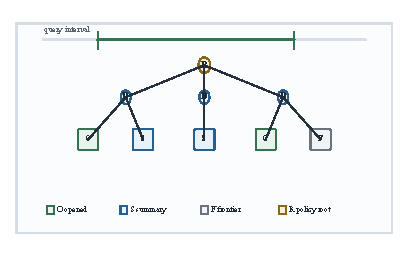
\includegraphics[width=\linewidth]{figs/index_certificate_flow.pdf}
\caption{Descriptor-bound physical design. Child intervals, counts, summary digests, and child hashes are authenticated together, so a pruned subtree cannot be relabeled as outside a query range.}
\label{fig:index}
\end{figure}

The design is a database index, not a black-box cryptographic proof. Fanout changes tree height and boundary cost. Summary granularity changes compactness and update cost. Key choice determines which predicates receive compact omission evidence. Score order supports top-k; date order supports range dashboards; a production system would maintain multiple authenticated projections or choose a primary proof contract per workload.

\subsection{Verifier Invariants}
The verifier enforces eight invariants, matching Table~\ref{tab:invariants}. Request binding checks that the certificate digest equals the client-visible contract, including the subject and purpose fields that select the manifest entry. Root binding checks the relation and manifest descriptors. Schema binding checks primary-key identity, required non-null integer verification attributes, descriptor-typed dimension attributes, strict numeric encodings, and release version. Descriptor typing recomputes every node hash from typed intervals, counts, summaries, and ordered child descriptors. Range cover rejects a hash-only object that overlaps the query range and rejects any compact cover whose descriptor interval is not fully contained in the requested range. Policy binding recompiles the manifest-derived predicate and projection. Result folding folds accepted contributions and compares them with the claimed result. Version binding checks that the relation and manifest releases are exactly the expected versions. The verifier has no trusted server-side predicate and no trusted server-side explanation.

The most important bug class is descriptor confusion. A Merkle tree implementation that authenticates only child hashes can accidentally let unauthenticated metadata travel beside the proof. In governed analytics that metadata includes intervals, policy summaries, and cardinalities. \sys therefore hashes the descriptor as a typed object. The adversarial suite includes a range-boundary relabeling attack that preserves a root hash but changes exposed interval metadata; the verifier rejects it because the descriptor no longer reconstructs.

\subsection{Certificate Generation}
Generation follows the same shape as ordinary query processing. The server first compiles the visible query and manifest entry into a governed operator contract. It then asks the authenticated index for a cover of the relevant key interval. For each fully covered node, it emits a summary object if the node's policy-cube dimensions are sufficient for the predicate; otherwise it opens the node recursively. For boundary nodes, it opens children until tuple membership can be decided. Finally, it emits the answer, the manifest evidence, the root descriptor, and the proof objects.


\begin{table}[t]
\centering
\caption{Verifier invariants. A certificate must pass all checks.}
\label{tab:invariants}
\scriptsize
\begin{tabular}{p{0.30\linewidth}p{0.60\linewidth}}
\toprule
Invariant & Check \\
\midrule
Request binding & Certificate query digest matches the client-requested contract. \\
Root binding & Relation root and manifest root match expected owner descriptor. \\
Schema binding & Primary-key identity, non-null verification and dimension attributes, and release version match the descriptor. \\
Descriptor typing & Node hashes are recomputed from intervals, counts, summaries, and ordered children. \\
Range cover & Hash-only objects must be disjoint; compact covers must be contained; boundary pages or tuples are opened exactly. \\
Policy binding & Predicate and projection are compiled from one manifest entry. \\
Result folding & Accepted leaves and summaries fold to the returned answer. \\
Version binding & Relation descriptor version and manifest release version match the committed owner descriptor. \\
\bottomrule
\end{tabular}
\end{table}

The generator is not trusted. It can choose a bad cover, emit too little evidence, or select an expensive evidence plan. The verifier is the trusted boundary. This matters because the same query processor can be optimized without changing the security argument: a faster generator is acceptable only if it still emits evidence satisfying the same invariants.

\subsection{Alternative Physical Layouts}
The contract is layout-independent. The artifact evaluates a fanout tree, a memory-bounded page cube, and an authenticated prefix cube. A prefix cube commits day-prefix policy summaries under a committed view root, proves a range by opening two index-addressed prefixes and subtracting them, and verifies only when the client supplies the expected committed view root together with the policy and relation descriptor digest; self-consistent but uncommitted prefix views, wrong prefix indices, and noncanonical integer encodings are rejected. A DBMS deployment could instead place descriptors beside pages, keep column-store projections for common predicate keys, or maintain separate roots for data-market products. These choices change build, update, storage, and proof costs, but not the verifier obligations: descriptor binding, policy binding, omission completeness, and result folding must still hold.

This boundary also rules out attractive shortcuts. A bare table hash authenticates a snapshot but not omitted authorized rows; the sound baseline below materializes the table and checks the digest before recomputing the governed query. Tuple proofs authenticate contributors but not completeness. A range tree without policy summaries cannot prove the governed slice. A policy log states an enforcement decision but not the returned computation. \sys's evaluated layouts keep these obligations checkable together.

\subsection{Updates and Versions}
For non-key updates, \sys modifies the leaf summary, recomputes the leaf digest, and repairs descriptors on the path to the root. The owner publishes the new root descriptor and manifest binding. Structural updates use version rebuilding: insert, delete, and key-update operations construct a new authenticated version and therefore preserve the same verifier contract. The evaluated versioned-update path provides optimized non-key repair when the key order is unchanged and certifiable rebuilding when the tree shape changes.

The version model is immutable at the verifier. A certificate is checked against an expected relation descriptor and manifest descriptor. Reusing an old root, substituting a neighboring manifest, or changing the version number changes the checked owner descriptor. This model supports auditability because the verifier can reproduce a decision from the version and manifest that were in force at release time.

\subsection{Evidence-Plan Boundary}
The generator is free to choose among evidence plans, but the verifier accepts only plans whose typed operator contract is implemented. This is the query-processing analogue of physical-plan legality: a summary cover, tuple/frontier proof, full witness, or opened-multiset join witness is admissible only when it supplies the required obligations, and it may not replace omission evidence with provenance or manifest binding with a policy log. The artifact compiles range group-by, AVG, HAVING, distinct, projection, row-local open scan, top-k, returned-pair join, complete FK join, anti-join, and many-to-many join templates to explicit obligations. The planner rejects candidates with missing obligations before ranking admissible plans by byte/time cost. Verification APIs are client-bound by default; self-certified checking remains only a negative-control mode, and a descriptor-only verifier checks compact group-by certificates without a server tree object.

\section{Evaluation}
\subsection{Questions and Setup}
The evaluation asks whether policy-carrying certificates stay compact, verification stays lightweight, attacks and partial baselines fail, efficiency scales with relation size, selectivity, policy complexity, and physical layout, richer operators remain certifiable, the contract survives profile shifts and public-tabular mappings, and trends hold across unused seeds. The scale suite uses several evidence paths: the full matrix uses 2K and 5K rows, compact-path stress reaches 20K and 50K, page-cube trends reach 1M rows, a 50K authenticated prefix-cube view measures materialized summaries, and a 100K star-schema-style profile checks skewed dashboard access. Five deterministic profile families, four unused seeds, four selectivities, and three policy complexities produce 240 robustness checks against the same verifier and SQLite oracle. Plotly Gapminder and 2014 Apple stock are bundled only as public-tabular distributional sanity checks~\cite{plotlygapminder,plotlyapple}.

Baselines are full recomputation, full table+hash materialization, tuple Merkle, tuple-plus-frontier, range tree, provenance-only, policy-oblivious proof, authenticated prefix-cube view, \sys summary proof, and an adaptive planner. The partial baselines are intentionally included to show where plausible shortcuts fail.

\subsection{Measurement Discipline}
All values come from deterministic CPU-only runs on an x86-64 Linux VM using CPython, SQLite, and matplotlib; the supplemental environment records the software stack. The measurements isolate verifier semantics, certificate-generation cost, physical evidence-plan trade-offs, update repair, and descriptor-only client verification under one reproducible implementation. Each run rebuilds seeded relations, generates manifests, executes governed queries, verifies certificates, and compares answers with an independent SQLite oracle over the authorized slice. Tables report medians across query settings, while stress, page-scale, prefix-cube, and robustness runs are reported separately to expose tails and memory behavior. Certificate sizes are canonical JSON bytes for every scheme, so compact, tuple, frontier, prefix-cube, and materialized baselines share one serialization path. Absolute timings are artifact measurements; the meaningful comparisons are paired within the same deterministic verifier/oracle run.

Cross-profile workloads stress different data-engineering shapes: dashboard sales, TPC-H-like skew, open-data permits, health-release summaries, finance-audit heavy tails, and two public CSV mappings. The robustness sweep reports median/p95 envelopes over all 240 verified settings rather than selecting one favorable seed.

\subsection{Efficiency, Scalability, and Verification Cost}
Table~\ref{tab:medians} summarizes median costs in the full baseline matrix. \sys's median certificate is 31.4 KiB with 3.64 ms generation and 1.98 ms verification. It is much smaller than tuple Merkle and tuple-plus-frontier in the median case, and orders of magnitude smaller than full materialization. Provenance-only is tiny, but it is unsound for omission; policy-oblivious is compact, but it cannot bind policy.

\begin{table}[t]
\centering
\caption{Median costs in the 2K--5K full-baseline matrix.}
\label{tab:medians}
\scriptsize
\begin{tabular}{p{0.38\linewidth}rrr}
\toprule
Scheme & Bytes & Verify ms & Gen. ms \\
\midrule
Provenance only & 385 & 0.001 & 0.43 \\
Policy-oblivious & 30,531 & 1.29 & 1.77  \\
\sys & 32,166 & 1.98 & 3.64  \\
Adaptive planner & 32,166 & 1.98 & 3.64  \\
Range tree & 59,732 & 1.78 & 2.22  \\
Tuple Merkle & 65,872 & 1.72 & 12.28  \\
Tuple plus frontier & 110,345 & 3.92 & 13.48  \\
Full recomputation & 505,512 & 0.33 & 0.01  \\
Full-table hash & 505,590 & 0.41 & 0.03  \\
\bottomrule
\end{tabular}
\end{table}

Fig.~\ref{fig:size} shows the largest full-baseline slice. Policy-cube summaries dominate tuple evidence for broader analytical ranges, while the adaptive planner can choose tuple-plus-frontier when that becomes smaller. Cost is separated from admissibility: compact provenance-only evidence is still excluded because it lacks omission completeness.

\begin{figure}[t]
\centering
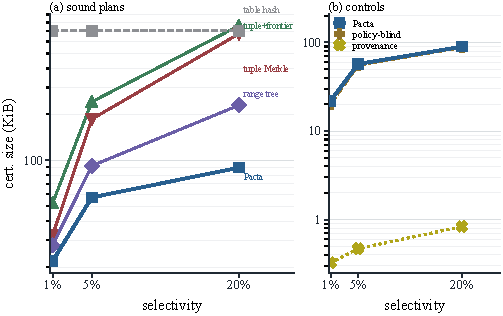
\includegraphics[width=\linewidth]{figs/cert_size_selectivity.pdf}
\caption{Certificate size versus selectivity. Negative controls are shown separately because compactness is not admissibility.}
\label{fig:size}
\end{figure}

Fig.~\ref{fig:time} gives compact-path scalability. Median verification is 1.67 ms at 2K rows, 2.63 ms at 5K, 4.04 ms at 20K, and 5.96 ms at 50K; generation rises from 2.66 ms to 10.91 ms, and the 50K median certificate remains 164.3 KiB. Cost follows the authenticated cover and touched policy cells rather than a full-table scan.

\begin{figure}[t]
\centering
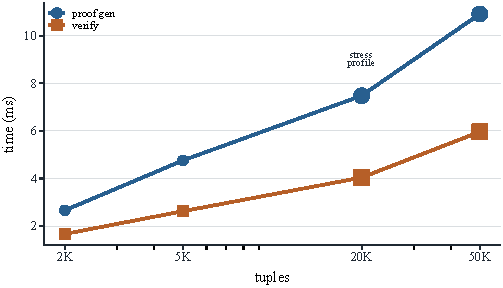
\includegraphics[width=\linewidth]{figs/time_scalability.pdf}
\caption{\sys proof generation and verification scalability. The 20K and 50K points are Pacta-only stress measurements.}
\label{fig:time}
\end{figure}

A page-cube experiment measures the same governed group-by contract at larger scale. It stores authenticated page summaries rather than one verifier object per tuple, uses compact page covers only for contained intervals, and opens boundary pages when a range cuts through a page. At 1M rows, the median certificate is 801.3 KiB, proof generation is 115.54 ms, descriptor-only verification is 84.83 ms, and the 489-page index builds in 4.77 s. Fig.~\ref{fig:large-scale} reports the 100K--1M trend. The strongest OLAP-style alternative is a materialized prefix cube: at 50K rows it gives 22.5 KiB certificates, 2.16 ms generation, and 2.89 ms verification, with a 1.14 s view-build cost and 500-prefix median update footprint. A 100K star-schema profile verifies 11.3 KiB prefix certificates in 1.34 ms.

\begin{figure}[t]
\centering
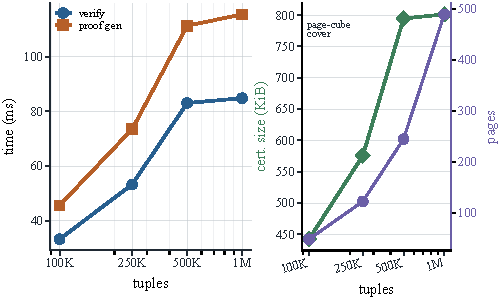
\includegraphics[width=\linewidth]{figs/large_scale_page_index.pdf}
\caption{Page-cube layout at large scale. Page summaries avoid tuple-object materialization without changing proof semantics.}
\label{fig:large-scale}
\end{figure}

\begin{table}[t]
\centering
\caption{Efficiency and scalability summary for verifier-checked certificate paths.}
\label{tab:scale}
\scriptsize
{\setlength{\tabcolsep}{2pt}
\begin{tabular}{@{}p{0.27\linewidth}p{0.16\linewidth}p{0.25\linewidth}p{0.22\linewidth}@{}}
\toprule
Path & Scale & Cert. / verify & Gen. or build \\
\midrule
Policy cube & 50K facts & 164.3 KiB / 5.96 ms & 10.91 ms gen. \\
Page cube & 1M facts & 801.3 KiB / 84.83 ms & 115.54 ms gen.; 4.77 s build \\
Prefix cube & 50K facts & 22.5 KiB / 2.89 ms & 2.16 ms gen.; 1.14 s build \\
Star prefix & 100K facts & 11.3 KiB / 1.34 ms & 0.90 ms gen. \\
Update repair & 5K tree & 960 B path & 4.43 ms vs. 225.11 ms rebuild \\
\bottomrule
\end{tabular}
}
\end{table}

\subsection{Attack Detection and Negative Controls}
Table~\ref{tab:detection} summarizes adversarial trials. \sys rejects tampered aggregates, replayed or stale catalogs, widened policies, manifest and projection-mask tampering, request/range mutation, descriptor tampering, hidden dimension or tag-policy changes, disclosure violations, omissions, and range-boundary relabeling. Provenance-only accepts omission because it lacks completeness evidence; policy-oblivious proof accepts widening because it has no manifest binding. The negative controls model common incomplete release artifacts.

\begin{table}[t]
\centering
\caption{Adversarial outcomes. Honest \sys certificates are accepted; all mutated \sys certificates are rejected.}
\label{tab:detection}
\scriptsize
\begin{tabular}{p{0.40\linewidth}p{0.20\linewidth}p{0.24\linewidth}}
\toprule
Trial & \sys detects & Weak accepts \\
\midrule
Tampered aggregate & Yes & -- \\
Stale or wrong version & Yes & -- \\
Policy filter widened & Yes & Yes \\
Manifest tampering & Yes & -- \\
Signed catalog replay/tamper & Yes & -- \\
Projection mask tampering & Yes & -- \\
Dimension/tag policy substitution & Yes & -- \\
Valid wrong-query certificate & Yes & Yes without request binding \\
Query range mutation & Yes & -- \\
Root descriptor tampering & Yes & -- \\
Omitted inside-range tuple & Yes & Yes \\
Count-distinct omission & Yes & -- \\
Anti-join hidden match & Yes & -- \\
Open-scan predicate or omission mutation & Yes & Compact inadmissible plan \\
Disclosure-contract violation & Yes & Unchecked opened evidence \\
Range-boundary relabeling & Yes & -- \\
Ambiguous JSON integer encoding & Yes & Lenient parser \\
\bottomrule
\end{tabular}
\end{table}

The deterministic randomized suite performs 240 SQLite semantic cross-checks across five synthetic workload profiles plus load checks for the two public CSV profiles. Operator tests cover request substitution, version and policy interval mutations, schema/null/duplicate errors, ambiguous encodings, count-distinct and projection omissions, anti-join and many-to-many omissions, AVG/HAVING mutations, open-scan predicate changes, top-k omissions, join request/segment binding, tag-policy substitution, and operator-field smuggling. Each check builds or maps a relation, compiles a manifest-derived policy, verifies a certificate, and compares the result with an independently evaluated SQLite query over the authorized slice.

\subsection{Updates, Top-k, Joins, and Workload Profiles}
Non-key update repair touches one leaf-to-root path: at 5K rows, median repair is 4.43 ms versus 225.11 ms for full rebuild. Insert, delete, and key-update version rebuilds cost 206.24 ms, 203.49 ms, and 215.40 ms. Derived-average and HAVING reuse the verified aggregate cover, while exact count-distinct opens the authorized multiset; complete range projection and count-distinct are 328.0 KiB/9.85 ms and 326.7 KiB/9.91 ms. The row-local predicate fallback is much larger, 2.95 MiB with 82.75 ms verification, because it authenticates every indexed-row candidate before applying an unsummarized amount predicate. Top-k is 107.4 KiB/3.50 ms for $k=20$; returned-pair drill-down joins are 105.8 KiB/2.87 ms. Complete FK, anti-join, and many-to-many contracts are 388.0 KiB/12.72 ms, 551.7 KiB/18.85 ms, and 298.5 KiB/10.38 ms, respectively. The pattern is compact reuse where summaries suffice and explicit witness cost where distinct and joins require completeness evidence.

Cross-profile medians show that the verifier is not tuned to one synthetic distribution. Compact certificates range from 43.0 KiB for finance-audit to 57.5 KiB for open-data permits; dashboard sales is 47.6 KiB, and TPC-H-like/open-data profiles touch larger ranges or more policy cells. The public Apple-stock and Gapminder mappings keep the same verifier and SQLite oracle while changing data shape. Fig.~\ref{fig:robust} reports the holdout sweep: across 240 fixed settings at 3K rows, compact certificates have median 39.8 KiB and p95 81.2 KiB, and client verification has median 2.27 ms and p95 3.30 ms.

\begin{figure}[t]
\centering
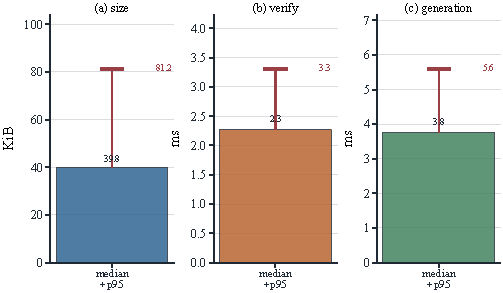
\includegraphics[width=\linewidth]{figs/robustness_sweep.pdf}
\caption{Holdout robustness sweep over unused seeds, profiles, selectivities, and policy complexities.}
\label{fig:robust}
\end{figure}

\subsection{Ablations and Design Lessons}
The central ablation is descriptor binding. If a proof authenticates only a subtree hash and carries interval metadata outside the hash, a malicious server can relabel a pruned overlapping subtree as outside the range. \sys rejects the range-boundary relabeling attack because intervals, counts, summary digests, and child hashes are jointly committed. Policy binding and omission evidence matter for the same reason: policy-oblivious proof accepts widening, and provenance-only evidence accepts an omitted inside-range tuple.

The best evidence shape is workload-dependent. Policy-cube summaries are compact for broad ranges with bounded policy dimensions; tuple-plus-frontier can win for tiny ranges; high-cardinality policies can make summaries grow. The evidence planner is therefore part of the contract, not only an optimization rule: every selected plan must satisfy the same verifier invariants.

\subsection{Cost Frontier}
The evaluation exposes a proof-size frontier rather than a single universal winner. For governed group-by, policy-cube summaries are 51.0 KiB at the planner-frontier median, while an equivalent open-range scan is 2.95 MiB; both are sound, but the summary is 59x smaller. With a prefix cube, the optimizer also has a 22.5 KiB materialized-view plan with 2.89 ms verification. For a row predicate over an uncommitted amount attribute, the 50.9 KiB summary is inadmissible because it lacks predicate-completeness evidence; the sound fallback is the 2.95 MiB open scan.

\begin{figure}[t]
\centering
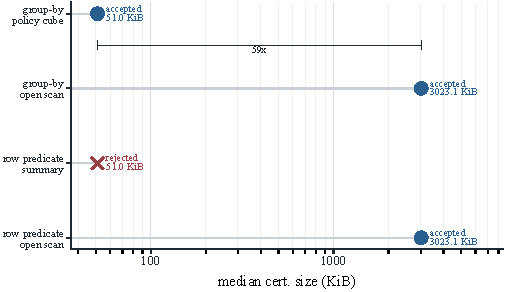
\includegraphics[width=\linewidth]{figs/planner_legality_frontier.pdf}
\caption{Certifying optimizer frontier. The optimizer ranks by cost only after the admissibility check.}
\label{fig:frontier}
\end{figure}

A release plan is admissible only if it satisfies the verifier contract; among admissible plans the system chooses by proof size, verification time, update cost, and release policy. The optimizer trace records accepted and rejected candidates, and Fig.~\ref{fig:frontier} reports the decision. The same fail-closed rule applies inside the typed IR: unsupported row predicates, HAVING clauses outside verified aggregate state, score-order fields on range operators, or returned-pair filters on completeness joins are rejected before proof generation.

\section{Related Work}
Authenticated data structures began with hash trees and query-oriented structures for outsourced databases~\cite{merkle1980protocols,devanbu2003authentic,martel2004model,tamassia2003ads,goodrich2001skip,anagnostopoulos2001persistent}. Authenticated database work studies completeness, aggregation, multidimensional queries, streams, spatial queries, top-k, joins, and dynamic data~\cite{pang2004edge,pang2005completeness,mykletun2004outsourced,sion2005assurance,narasimha2006signature,li2006dynamic,li2010aggregation,cheng2006multidimensional,li2007streams,papadopoulos2009sae,yang2009join,mouratidis2009spatial,papadopoulos2010streams,chen2013topk,chen2015integration,bajaj2019concurrent}. ServeDB and VeriDB bring verifiability closer to database deployments through secure range queries and enclave-backed verification~\cite{zhou2019servedb,li2021veridb}. \sys builds on this line but verifies a manifest-derived authorized slice, and makes plan admissibility a query-processor obligation.

Verifiable computation and encrypted databases provide stronger or different guarantees~\cite{benabbas2011vdelegation,setty2012pepper,parno2013pinocchio,zhang2017vsql,hacigumus2002encrypted,popa2011cryptdb,zheng2017opaque}. \sys is complementary: it offers an operator-aware database contract whose verifier sees the request digest, manifest binding, projection mask, omission evidence, and physical evidence shape.

Policy-aware databases, fine-grained authorization, purpose-based access control, privacy systems, and differential privacy define or enforce access~\cite{stonebraker1974access,agrawal2002hippocratic,agrawal2005privacy,rizvi2004fgac,kabra2006fgac,chaudhuri2007predicated,byun2008purpose,colombo2015action,sandhu1996rbac,jajodia1997multipolicy,mcsherry2009pinq,dwork2006dp,paduroiu2024sparkaccess}; \sys checks that the compiled policy was used in the result. Provenance and accountability explain contributors or record behavior~\cite{cui2000lineage,buneman2001whywhere,green2007semiring,cheney2009provenance,karvounarakis2010provenance,glavic2007categorization,herschel2017survey,glavic2021provenance,meliou2010causality,amsterdamer2011provenance,haeberlen2007peerreview}, but do not prove omission completeness or prevent a widened manifest.

Physical design determines verification cost. Aggregate processing, data cubes, materialized views, B-trees, synopses, column stores, Dremel, and Spark SQL show how layout and summaries govern analytical performance~\cite{chaudhuri1994aggregate,gray1997datacube,harinarayan1996cubes,gupta1993views,graefe2011btree,cormode2012synopses,abadi2006columnstores,melnik2010dremel,armbrust2015sparksql}. Data-product pipelines, dataspaces, collaborative dataset systems, programmable sharing, and data-market platforms motivate the sharing setting~\cite{polyzotis2017data,franklin2005dataspaces,bhardwaj2015datahub,fernandez2020datahub,pei2023markets,xia2026sharing}. \sys connects the two threads by asking which physical evidence plan can certify the governed result a client is allowed to receive.


\section{System Implications and Conclusion}
\sys treats governed analytical verification as physical design under verifier obligations. A query processor may change indexes, summaries, and execution strategies only when the emitted evidence proves the same request-bound, schema-bound, manifest-derived authorized-bag computation. The owner publishes descriptors and manifest roots; the client sends a typed governed request; the server returns an answer and certificate; and the verifier checks descriptors, manifest-derived predicates/projections, authenticated covers, and folded results. Compact summaries, tuple/frontier proofs, opened ranges, opened multisets, top-k accumulators, join witnesses, signed catalogs, leakage contracts, prefix views, and page descriptors are ranked only after admissibility is established.

The result is a reusable contract between storage, policy, and query processing for data products, clean rooms, audit dashboards, and marketplaces. Table~\ref{tab:scope} defines the accepted analytical contracts, and unsupported requests either compile to opened evidence with the required attributes or fail closed before proof generation. The artifact makes the contract falsifiable: every number has a certificate shape, every certificate has a verifier obligation, every negative control explains an unsafe shortcut, and every scale path preserves the same client-checkable governed answer object.

For a database implementer, the practical message is that verifiability should be planned at the same layer as physical design. A secondary index, cube, prefix view, or opened scan is not merely an access path; it is a proposal about which facts the client can later check. This changes optimizer bookkeeping. The optimizer must carry obligation types, committed descriptor fields, and disclosure contracts beside byte and time estimates. Once those fields are explicit, conventional engineering choices still apply: a deployment can cache descriptors, choose fanout, maintain multiple projections, or materialize a prefix cube. What cannot be hidden is the reason a chosen evidence plan proves the governed answer.

For a data-product owner, the separation between policy enforcement and certificate verification is equally important. \sys does not ask the verifier to judge whether a policy is legally correct, nor does it replace the owner's authorization engine. Instead, it records the compiled manifest, projection mask, release version, and descriptor roots as the public boundary of the result. The owner may revise policy, rotate keys, publish a new catalog, or attach richer release metadata, but each accepted answer remains tied to one concrete release contract. This makes stale policy, broader tenant scope, and accidental projection drift observable to clients rather than buried inside server logs.

The evaluation also argues for negative controls as first-class systems evidence. Compact certificates are persuasive only when nearby cheap but unsound artifacts fail in predictable ways. The policy-oblivious and provenance-only baselines are not weak because they are poorly implemented; they are weak because their object of authentication is smaller than the governed query contract. Likewise, the planner frontier is useful because it distinguishes an admissible compact summary from a compact row-predicate shortcut that omits the committed predicate attribute. This style of experiment makes the theorem boundary operational: every accepted optimization has a matching verifier obligation, and every rejected shortcut names the missing one.

The current boundary is intentionally conservative. It does not certify arbitrary SQL, hidden UDF semantics, differential privacy, confidential computation, or the organizational validity of the underlying policy. Those mechanisms can be layered around the contract, but the certificate itself checks the database facts it is designed to check: request binding, descriptor reconstruction, manifest-derived authorization, omission completeness, duplicate handling, projection safety, freshness, and result folding. Keeping that boundary narrow is a strength for auditability. It prevents a release artifact from implying broader privacy, legal, or semantic guarantees than the verifier actually tests.

This perspective leaves several engineering directions without changing the core contract. A production system could maintain descriptor families for multiple physical layouts, expose cost estimates to owners before publication, or precompute prefix views for frequent governed dashboards. A query compiler could surface inadmissible requests with the missing committed attributes, turning fail-closed planning into feedback for schema and policy design. Distributed settings would require catalog replication and version discipline, but not a different proof object: each shard can still contribute descriptors, summary cells, opened witnesses, and freshness evidence that fold into the same governed answer.

The broader conclusion is that governed analytics needs a client-checkable answer object, not only authentic rows or explanatory provenance. Once the answer object includes the query, manifest, projection, descriptor version, and evidence plan, database physical design becomes accountable to the policy boundary. \sys shows that this accountability is compatible with compact summaries and ordinary SQL-style operators when the verifier obligations are typed and enforced before cost ranking. The result is a portable systems pattern: make the governed contract explicit, let the optimizer search only within that contract, and report costs only for evidence plans the client can independently reject or accept.

Two details are worth preserving in future extensions. First, proof objects should remain inspectable by a verifier that does not replay the service's planner or trust its catalog cache. This is why descriptors, policy roots, opened witnesses, and folded aggregates are explicit certificate fields rather than implicit server state. Second, performance claims should remain conditional on verifier obligations. A faster plan is not a better plan if it changes the disclosure contract, drops an omission witness, or authenticates a weaker predicate than the request committed. Treating admissibility as a typed planning precondition keeps the empirical comparison honest: compactness is measured only after the plan proves the right answer object.

Those constraints also make \sys a database contribution rather than only a cryptographic wrapper. The work is not to attach a proof after execution, but to make physical design, operator choice, and result folding visible to the same contract the client checks. Conventional machinery remains useful only with explicit answer-boundary obligations.

\clearpage
\section*{Acknowledgments}
AI-generated content acknowledgement: The authors used AI only for language and grammar polishing.

\bibliographystyle{IEEEtran}
\bibliography{references}

\end{document}
